\documentclass[a4paper,12pt]{report}

\usepackage{alltt, fancyvrb, url}
\usepackage{graphicx}
\usepackage[utf8]{inputenc}
\usepackage{float}
\usepackage{hyperref}

% Questo commentalo se vuoi scrivere in inglese.
\usepackage[italian]{babel}

\usepackage[italian]{cleveref}

\title{Relazione per \\``Programmazione ad Oggetti'' \\ \\Progetto ''Unibo-td''}

\author{Aurora Francesco, Casali Marco, Murvai Cristina, Pulga Luca}
\date{04 luglio 2024}


\begin{document}

\maketitle

\begin{abstract}
Questa relazione descrive lo sviluppo del progetto "Unibo TD", un gioco di tipo tower defense, utilizzando il pattern architetturale MVC (Model-View-Controller). Lo scopo di questo documento è fornire una guida dettagliata sul processo di sviluppo, evidenziando i principali punti da trattare e come farlo in modo efficace, evitando di soffermarsi su aspetti marginali e concentrandosi su quelli di maggiore rilevanza.
\end{abstract}

\begin{figure}[H]
    \centering
    \includegraphics[width=\textwidth]{intro.jpg}
    \caption{Schermata di un tipico gioco Tower-Defense}
    \label{fig:enter-label}
\end{figure}

\tableofcontents

\chapter{Analisi}

Questo documento fornisce una panoramica dei requisiti fondamentali per lo sviluppo del gioco Tower-Defense ispirato a Bloons TD. I requisiti tecnici dettagliati e le specifiche implementative saranno trattati in fasi successive del processo di sviluppo, mantenendo il focus sul comportamento e le funzionalità dell'applicazione.

\section{Requisiti}

L'obiettivo del presente documento è definire i requisiti dell'applicazione per il gioco di tipo Tower-Defense ispirato a Bloons TD. Questo gioco sarà progettato per offrire un'esperienza coinvolgente simile al gioco di riferimento, adattata alle specifiche del progetto.

\subsection*{Requisiti funzionali}
\begin{itemize}
	\item Un gioco di tipo Tower Defense è un genere in cui i giocatori devono posizionare torri strategiche lungo un percorso per fermare onde di nemici. Le torri, ciascuna con abilità specifiche, devono essere posizionate strategicamente per prevenire che i nemici raggiungano un punto finale, solitamente la base o un obiettivo.
	\item Deve essere possibile avviare un nuovo gioco e visualizzare informazioni essenziali come punteggi e stato del gioco.
	\item Dividere il gioco in round con difficoltà incrementale.
	\item Creare una mappa giocabile con percorsi definiti per i nemici.
	\item Gli utenti devono poter piazzare diverse torri lungo il percordo di gioco per difendersi dai nemici.
	\item Le torri devono essere posizionabili in punti specifici del campo.
	\item Ogni difesa deve avere esattamente una arma utilizzabile.
	\item Deve essere possibile avviare un nuovo gioco e visualizzare informazioni essenziali come punteggi e stato del gioco.
	\item Gestire le interazioni tra i nemici e le difese, inclusi attacchi e difese delle torri.
	\item Gestire un sistema di vite limitate per i giocatori; il gioco termina quando le vite si esauriscono.
	\item Implementare un sistema di gestione economica per guadagnare e spendere monete nelle difese.
\end{itemize}

\subsection*{Requisiti non funzionali}
\begin{itemize}
	\item Garantire fluidità del gioco su diverse piattaforme, con un'attenzione particolare alla velocità di caricamento dei livelli e all'ottimizzazione generale.
	\item Assicurare che il gioco sia compatibile con dispositivi desktop supportando almeno le versioni recenti dei principali sistemi operativi (windows, linux, macos).
	\item Il linguaggio di porgrammazione adottato sarà Java
\end{itemize}

\section{Analisi e modello del dominio}

Unibo TD avrà più entità che dovranno collaborare tra loro.

\subsection*{Gestione delle difese}
\begin{itemize}
Il gioco sarà costituito da una mappa. All'interno della mappa saranno presenti delle celle edificabili su cui poter posizionare le proprie difese (\textit{torri}). 
Le difese sono le unità incaricate a proteggere il punto terminale della mappa. Queste saranno quindi in grado di infliggere danni ai nemici attraverso specifiche logiche di targettamento e di attacco. Ogni tipologia difesa possiederà certe statistiche per poter garantire maggiore eterogeneità al gioco. Per costruire una difesa sarà necessaria una certa quantità di denaro, acquisibile tramite l'eliminazione di nemici nei vari round. Ogni difesa oltre ad avere relative speficifiche e caratteristiche, fra queste figurano anche le \textit{armi} a disposizione di ogni torre, le quali gestiscono la \textit{frequenza} di sparo dei \textit{proiettili} per arrecare danno ai nemici. Ogni proiettile sparato da una determinata torre con una determinata arma, dispone di un certo danno. Ogni qualvolta una difesa sconfigge un nemico, verrà accreditato al \textbf{player} il denaro relativo al nemico sconfitto. Due feature interessanti sarebbero la rimozione e il riposizionamento delle difese sulla mappa nei punti permessi. Queste purtroppo non potranno essere effettuate all’interno del monte ore previsto e conseguentemente si rimanda tale feature in futuro.
\end{itemize}

\chapter{Design}

\section{Architettura}

L'architettura dell'applicazione sviluppata si basa sul modello architetturale MVC (Model-Controller-View). Il Model, una volta avviato dal Controller, esternalizza e gestisce in modo trasparente la logica tramite il defense manager e l'enemy manager, i quali si occupano di aspetti diversi del gioco, come i nemici e le difese. Il Controller funge da intermediario tra Model e View, limitando l'accesso diretto al Model e fornendo solo oggetti di trasferimento dati. Ciò significa che gli altri componenti dell'applicazione, come la View, possono accedere solo a una rappresentazione immutabile dei dati nel Model, garantendo un maggiore controllo sull'integrità dei dati. Di conseguenza, l'implementazione della View, così come è stata definita, è facilmente sostituibile poiché non dipende dalle classi sottostanti.
\begin{figure}
    \centering
    
\includegraphics[width=0.5\linewidth]{todo.jpg}
    \caption{Figura 2.1: Architettura MVC}
    \label{fig:enter-label}
\end{figure}
\section{Design dettagliato}
\textbf{Luca Pulga}
\subsection{Gestione delle difese}

\textbf{Problema}:
Si vuole gestire in maniera scalabile le varie entità presenti all'interno del gioco, come le difese (torri, armi, proiettili) e i nemici, evitando l'eccessiva scrittura di codice duplicato.

\textbf{Soluzione}:
E' possibile suddividere le varie caratteristiche delle varie entità in sotto-entità, in modo da attribuire le relative proprietà ad ogni tipologia di entità che è presente
o che potrà essere presente in futuro, rendendo la struttura scalabile. Sono state realizzate interfacce e classi astratte, a cui sono state delegate le assegnazioni delle varie proprietà fornendo la condivisione del codice comune e contratti parziali, implementabili dalle sottoclassi.
Un'ulteriore soluzione poteva essere quella di utilizzare solo interfacce e come implementazione di esse, utilizzare i record, in quanto fornirebbero un modo decisamente più coinciso per dichiarare classi immutabili ed eliminerebbero molta della verbosità associata alle classi standard.

\begin{figure}[H]
    \centering
    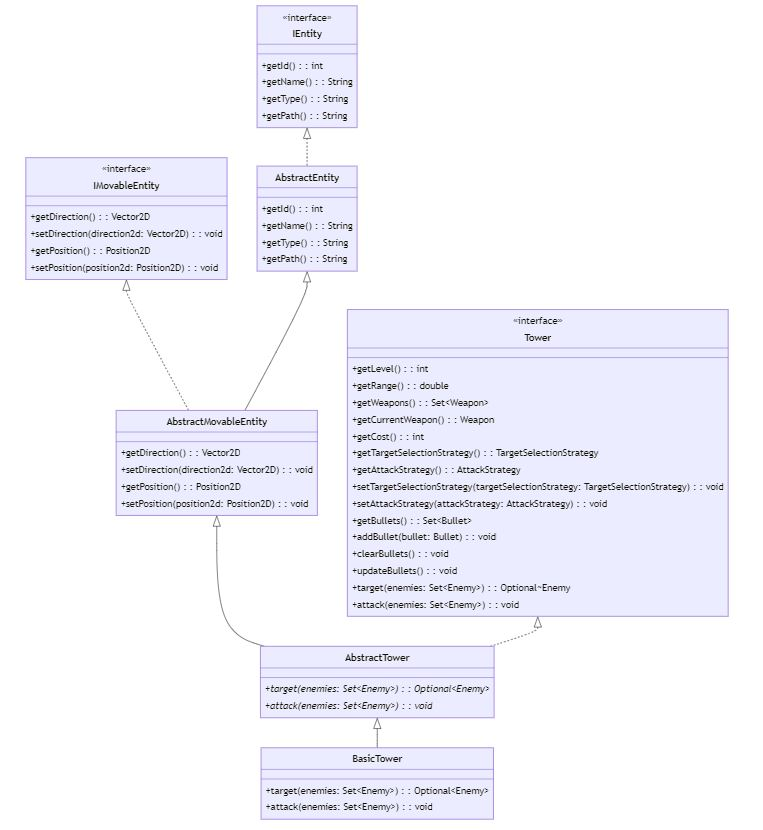
\includegraphics[width=1.2\linewidth]{defense_model.JPG}
    \caption{Figura 2.2: Modello per la gestione delle entità.}
    \label{fig:defense-model}
\end{figure}

\textbf{Problema}:
Disporre di un oggetto in grado di poter creare qualsiasi tipo di entità, centralizzando la parte di creazione degli oggetti che verranno caricati e successivamente utilizzati
durante il gioco.

\textbf{Soluzione}:
Viene utilizzato il \textit{Factory Method Pattern} in modo da sfruttare la sua capacità di separare la costruzione degli oggetti dal loro utilizzo. Dunque questa separazione ci consente di avere una maggiore flessibilità e modularità del codice, rendendolo più facile da mantenere e aggiornare anche introducendo in futuro nuove entità o separare in sotto-entità quelle già esistenti. 
La \textit{Factory} provvederà a leggere i file json all'interno di specifiche cartelle per caricare
le entità, come le \textit{torri}, che saranno poi successivamente gestite dal \textit{Defense Manager}.
\begin{figure}[H]
    \centering
    \includegraphics[width=0.8\linewidth]{entity-factory-method.jpg}
    \caption{Figura 2.3: Factory Method Pattern per il caricamento delle entità.}
    \label{fig:entity-factory-method}
\end{figure}

\textbf{Problema}:
Gestione delle istanze delle torri senza avere un'entità centralizzata.
\textbf{Soluzione}:
La soluzione prevedere l'implementazione di un Defense Manager in grado di gestire le entità difesa. Questa soluzione centralizzata permette di gestire all'interno di un unica classe tutte le entità difesa, fornendo anche un modo comodo all'esterno per ottenere informazioni con altri oggetti.

\begin{figure}[H]
    \centering
    \includegraphics[width=0.8\linewidth]{defense-manager.jpg}
    \caption{Figura 2.4: Defense Manager per la gestione delle difese.}
    \label{fig:defense-manager}
\end{figure}


\textbf{Problema}:
Implementazione Observer.
\textbf{Soluzione}:


\begin{figure}[H]
    \centering
    \includegraphics[width=0.8\linewidth]{defense-observer.jpg}
    \caption{Figura 2.5: Defense Manager e Observer.}
    \label{fig:defense-observer}
\end{figure}

\textbf{Problema}:
Implementazione di diverse tipologie di targettamento dei nemici da parte delle torri a seconda della loro tipologia.
\textbf{Soluzione}:
Si implementa il Pattern Strategy, in questo modo il contesto diventa indipendente dalle strategie concrete di targettamento dei nemici, per cui è possibile aggiungere/modificare gli algoritmi di targettamento senza modificare il codice all'interno delle varie classi che potrebbero implementare la relativa strategia di attacco.


\begin{figure}[H]
    \centering
    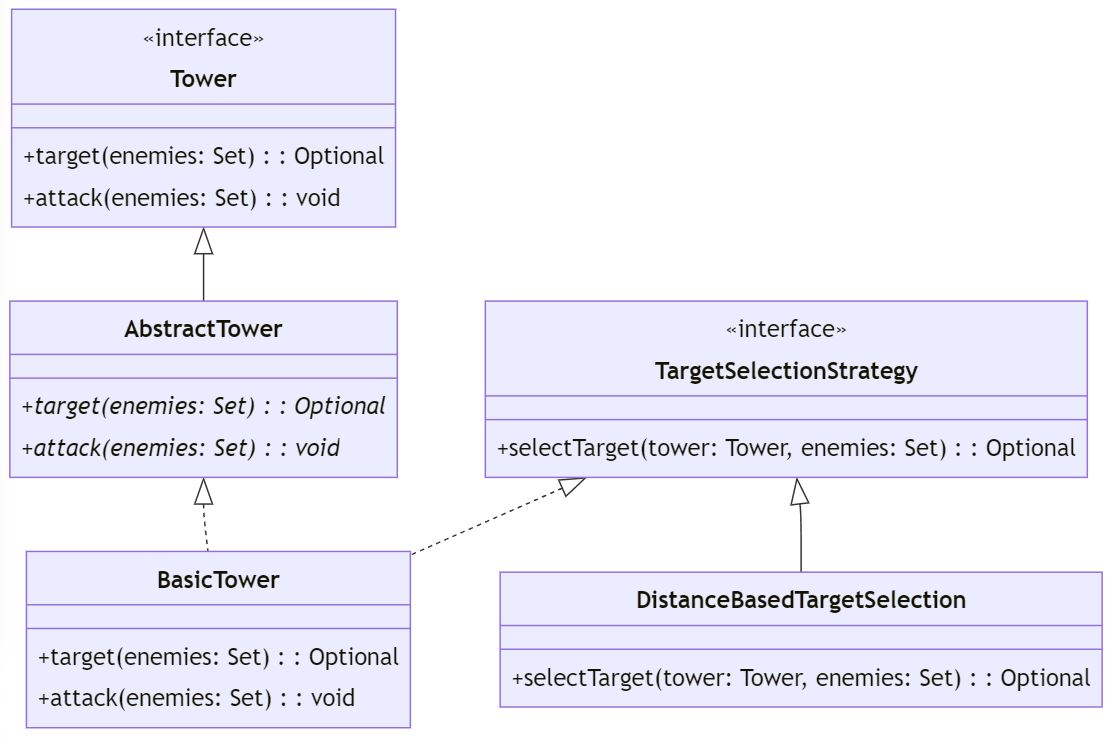
\includegraphics[width=0.8\linewidth]{defense_target.JPG}
    \caption{Figura 2.6: Pattern Strategy per targettamento dei nemici.}
    \label{fig:defense_target}
\end{figure}



\textbf{Problema}:
Implementazione di diverse tipologie di attacchi verso i nemici da parte delle torri a seconda della loro tipologia.
\textbf{Soluzione}:
Si implementa il Pattern Strategy, in questo modo il contesto diventa indipendente dalle strategie concrete di attacco verso i nemici, per cui è possibile aggiungere/modificare gli algoritmi di attacco senza modificare il codice all'interno delle varie classi che potrebbero implementare la relativa strategia di attacco.

\begin{figure}[H]
    \centering
    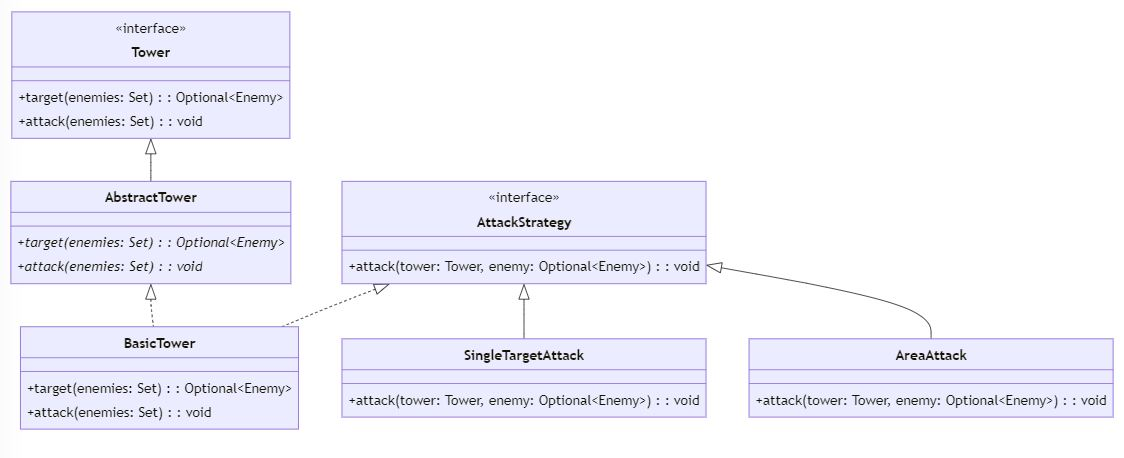
\includegraphics[width=0.8\linewidth]{defense_attack.JPG}
    \caption{Figura 2.7: Pattern Strategy per attacco ai nemici.}
    \label{fig:defense_attack}
\end{figure}


\chapter{Sviluppo}
\section{Testing automatizzato}
Per verificare il corretto funzionamento del gioco Tower-Defense, sono stati creati appositi test automatizzati utilizzando JUnit. 
I test automatizzati sono necessari per poter testare se le logiche pensate durante la fase analisi, di progettazione e di implementazione del Model, e delle classi affini di utility, sono funzionanti.

\begin{itemize}
    \item \textit{\textbf{TestBasicTower}:} Test automatizzato per garantire la correttezza dei metodi di get e set delle difese torri per poter gestire durante il gioco le sue proprietà.
    \item \textit{\textbf{TestBulletImpl}:} Test automatizzato per garantire la correttezza dei metodi di get e set della posizione e direzione del proiettile, fondamentale per la gestione grafica del gioco.
    \item \textit{\textbf{TestDefenseFactory}:} Test automatizzato per garantire la correttezza di lettura da file json delle entità torri attraverso l'utilizzo della \ref{fig:entity-factory-method}EntityFactory
    \item \textit{\textbf{TestTargetStrategy}:} Test automatizzato per garantire la correttezza dei calcoli effettuati durante la fase di targettamento di nemici da parte delle torri.
\end{itemize}

\section{Note di sviluppo}

Questa sezione, come quella riguardante il design dettagliato va svolta \textbf{singolarmente da ogni membro del gruppo}.
%
Nella prima parte, ciascuno dovrà mostrare degli esempi di codice particolarmente ben realizzati,
che dimostrino proefficienza con funzionalità avanzate del linguaggio e capacità di spingersi oltre le librerie mostrate a lezione.

\begin{itemize}
	\item \textbf{Elencare} (fare un semplice elenco per punti, non un testo!) le feature \textit{avanzate} del linguaggio e dell'ecosistema Java che sono state
utilizzate. Le feature di interesse sono:
	\begin{itemize}
		\item Progettazione con generici, ad esempio costruzione di nuovi tipi generici, e uso di generici bounded.
		L'uso di classi generiche di libreria non è considerato avanzato.
		\item Uso di lambda expressions
		\item Uso di \texttt{Stream}, di \texttt{Optional} o di altri costrutti funzionali
		\item Uso di reflection
		\item Definizione ed uso di nuove annotazioni
		\item Uso del Java Platform Module System
		\item Uso di parti della libreria JDK non spiegate a lezione (networking, compressione, parsing XML, eccetera...)
		\item Uso di librerie di terze parti (incluso JavaFX): Google Guava, Apache Commons...
	\end{itemize}
	\item Si faccia molta attenzione a non scrivere banalità, elencando qui features di tipo ``core'', come le eccezioni, le enumerazioni, o le inner class: nessuna di queste è considerata avanzata.
	\item Per ogni feature avanzata, mostrata, includere:
	\begin{itemize}
		\item Nome della feature
		\item Permalink GitHub al punto nel codice in cui è stata utilizzata
	\end{itemize}
\end{itemize}

In questa sezione, \textit{dopo l'elenco},
vanno menzionati ed attributi con precisione eventuali pezzi di codice ``riadattati'' (o scopiazzati...) da Internet o da altri progetti,
pratica che tolleriamo ma che non raccomandiamo.
%
Si rammenta agli studenti che non è consentito partire da progetti esistenti e procedere per modifiche successive.
%
Si ricorda anche che i docenti hanno in mano strumenti antiplagio piuttosto raffinati e che ``capiscono'' il codice e la storia delle modifiche del progetto,
per cui tecniche banali come cambiare nomi (di classi, metodi, campi, parametri, o variabili locali),
aggiungere o togliere commenti,
oppure riordinare i membri di una classe vengono individuate senza problemi.
%
Le regole del progetto spiegano in dettaglio l'approccio dei docenti verso atti gravi come il plagiarismo.

I pattern di design \textbf{non} vanno messi qui.
%
L'uso di pattern di design (come suggerisce il nome) è un aspetto avanzato di design, non di implementazione,
e non va in questa sezione.

\subsection*{Elementi positivi}

\begin{itemize}
	\item Si elencano gli aspetti avanzati di linguaggio che sono stati impiegati
	\item Si elencano le librerie che sono state utilizzate
	\item Per ciascun elemento, si fornisce un permalink
	\item Ogni permalink fa riferimento ad uno snippet di codice scritto dall'autore della sezione (i docenti verificheranno usando \texttt{git blame})
	\item Se si è utilizzato un particolare algoritmo, se ne cita la fonte originale.
	Ad esempio, se si è usato Mersenne Twister per la generazione di numeri pseudo-random, si cita \cite{mersenne}.
	\item Si identificano parti di codice prese da altri progetti, dal web, o comunque scritte in forma originale da altre persone.
	In tal senso, si ricorda che agli ingegneri non è richiesto di re-inventare la ruota continuamente:
	se si cita debitamente la sorgente è tollerato fare uso di di snippet di codice open source per risolvere velocemente problemi non banali.
	Nel caso in cui si usino snippet di codice di qualità discutibile,
	oltre a menzionarne l'autore originale si invitano gli studenti ad adeguare tali parti di codice agli standard e allo stile del progetto.
	Contestualmente, si fa presente che è largamente meglio fare uso di una libreria che copiarsi pezzi di codice:
	qualora vi sia scelta (e tipicamente c'è), si preferisca la prima via.
\end{itemize}

\subsection*{Elementi negativi}
\begin{itemize}
	\item Si elencano feature core del linguaggio invece di quelle segnalate. Esempi di feature core da non menzionare sono:
    \begin{itemize}
        \item eccezioni;
        \item classi innestate;
        \item enumerazioni;
        \item interfacce.
    \end{itemize}
	\item Si elencano applicazioni di terze parti (peggio se per usarle occorre licenza, e lo studente ne è sprovvisto) che non c'entrano nulla con lo sviluppo, ad esempio:
    \begin{itemize}
        \item Editor di grafica vettoriale come Inkscape o Adobe Illustrator;
        \item Editor di grafica scalare come GIMP o Adobe Photoshop;
        \item Editor di audio come Audacity;
        \item Strumenti di design dell'interfaccia grafica come SceneBuilder: il codice è in ogni caso inteso come sviluppato da voi.
    \end{itemize}
	\item Si descrivono aspetti di scarsa rilevanza, o si scende in dettagli inutili.
	\item Sono presenti parti di codice sviluppate originalmente da altri che non vengono debitamente segnalate.
	In tal senso, si ricorda agli studenti che i docenti hanno accesso a tutti i progetti degli anni passati,
	a Stack Overflow,
	ai principali blog di sviluppatori ed esperti Java,
	ai blog dedicati allo sviluppo di soluzioni e applicazioni
	(inclusi blog dedicati ad Android e allo sviluppo di videogame),
	nonché ai vari GitHub, GitLab, e Bitbucket.
	Conseguentemente, è \emph{molto} conveniente \emph{citare} una fonte ed usarla invece di tentare di spacciare per proprio il lavoro di altri.
	\item Si elencano design pattern
\end{itemize}

\subsection{Esempio}

\subsubsection{Utilizzo della libreria SLF4J}

Utilizzata in vari punti.
Un esempio è \url{https://github.com/AlchemistSimulator/Alchemist/blob/5c17f8b76920c78d955d478864ac1f11508ed9ad/alchemist-swingui/src/main/java/it/unibo/alchemist/boundary/swingui/effect/impl/EffectBuilder.java#L49}

\subsubsection{Utilizzo di \texttt{LoadingCache} dalla libreria Google Guava}

Permalink: \url{https://github.com/AlchemistSimulator/Alchemist/blob/d8a1799027d7d685569e15316a32e6394632ce71/alchemist-incarnation-protelis/src/main/java/it/unibo/alchemist/protelis/AlchemistExecutionContext.java#L141-L143}

\subsubsection{Utilizzo di \texttt{Stream} e lambda expressions}

Usate pervasivamente. Il seguente è un singolo esempio.
Permalink: \url{https://github.com/AlchemistSimulator/Alchemist/blob/d8a1799027d7d685569e15316a32e6394632ce71/alchemist-incarnation-protelis/src/main/java/it/unibo/alchemist/model/ProtelisIncarnation.java#L98-L120}

\subsubsection{Scrittura di metodo generico con parametri contravarianti}

Permalink: \url{https://github.com/AlchemistSimulator/Alchemist/blob/d8a1799027d7d685569e15316a32e6394632ce71/alchemist-incarnation-protelis/src/main/java/it/unibo/alchemist/protelis/AlchemistExecutionContext.java#L141-L143}

\subsubsection{Protezione da corse critiche usando \texttt{Semaphore}}

Permalink: \url{https://github.com/AlchemistSimulator/Alchemist/blob/d8a1799027d7d685569e15316a32e6394632ce71/alchemist-incarnation-protelis/src/main/java/it/unibo/alchemist/model/ProtelisIncarnation.java#L388-L440}


\chapter{Commenti finali}

In quest'ultimo capitolo si tirano le somme del lavoro svolto e si delineano eventuali sviluppi
futuri.

\textit{Nessuna delle informazioni incluse in questo capitolo verrà utilizzata per formulare la valutazione finale}, a meno che non sia assente o manchino delle sezioni obbligatorie.
%
Al fine di evitare pregiudizi involontari, l'intero capitolo verrà letto dai docenti solo dopo aver formulato la valutazione.

\section{Autovalutazione e lavori futuri}

\textbf{È richiesta una sezione per ciascun membro del gruppo, obbligatoriamente}.
%
Ciascuno dovrà autovalutare il proprio lavoro, elencando i punti di forza e di debolezza in quanto prodotto.
Si dovrà anche cercare di descrivere \emph{in modo quanto più obiettivo possibile} il proprio ruolo all'interno del gruppo.
Si ricorda, a tal proposito, che ciascuno studente è responsabile solo della propria sezione: non è un problema se ci sono opinioni contrastanti, a patto che rispecchino effettivamente l'opinione di chi le scrive.
Nel caso in cui si pensasse di portare avanti il progetto, ad esempio perché effettivamente impiegato, o perché sufficientemente ben riuscito da poter esser usato come dimostrazione di esser capaci progettisti, si descriva brevemente verso che direzione portarlo.

\section{Difficoltà incontrate e commenti per i docenti}

Questa sezione, \textbf{opzionale}, può essere utilizzata per segnalare ai docenti eventuali problemi o difficoltà incontrate nel corso o nello svolgimento del progetto, può essere vista come una seconda possibilità di valutare il corso (dopo quella offerta dalle rilevazioni della didattica) avendo anche conoscenza delle modalità e delle difficoltà collegate all'esame, cosa impossibile da fare usando le valutazioni in aula per ovvie ragioni.
%
È possibile che alcuni dei commenti forniti vengano utilizzati per migliorare il corso in futuro: sebbene non andrà a vostro beneficio, potreste fare un favore ai vostri futuri colleghi.
%
Ovviamente \textit{il contenuto della sezione non impatterà il voto finale}.

\appendix
\chapter{Guida utente}

Capitolo in cui si spiega come utilizzare il software. Nel caso in cui il suo uso sia del tutto
banale, tale capitolo può essere omesso.
%
A tal riguardo, si fa presente agli studenti che i docenti non hanno mai utilizzato il software
prima, per cui aspetti che sembrano del tutto banali a chi ha sviluppato l'applicazione possono non
esserlo per chi la usa per la prima volta.
%
Se, ad esempio, per cominciare una partita con un videogioco è necessario premere la barra
spaziatrice, o il tasto ``P'', è necessario che gli studenti lo segnalino.

\subsection*{Elementi positivi}

\begin{itemize}
 \item Si istruisce in modo semplice l'utente sull'uso dell'applicazione, eventualmente facendo uso di schermate e descrizioni.
\end{itemize}

\subsection*{Elementi negativi}
\begin{itemize}
 \item Si descrivono in modo eccessivamente minuzioso tutte le caratteristiche, anche minori, del software in oggetto.
 \item Manca una descrizione che consenta ad un utente qualunque di utilizzare almeno le funzionalità primarie dell'applicativo.
\end{itemize}

\chapter{Esercitazioni di laboratorio}

In questo capitolo ciascuno studente elenca gli esercizi di laboratorio che ha svolto
(se ne ha svolti),
elencando i permalink dei post sul forum dove è avvenuta la consegna.
%
Questa sezione potrebbe essere processata da strumenti automatici,
per cui link a oggetti diversi dal permalink della consegna,
errori nell'email o nel nome del laboratorio possono portare ad ignorare alcune consegne,
si raccomanda la massima precisione.

\section*{Esempio}

\subsection{paolino.paperino@studio.unibo.it}

\begin{itemize}
 \item Laboratorio 04: \url{https://virtuale.unibo.it/mod/forum/discuss.php?d=12345#p123456}
 \item Laboratorio 06: \url{https://virtuale.unibo.it/mod/forum/discuss.php?d=22222#p222222}
 \item Laboratorio 09: \url{https://virtuale.unibo.it/mod/forum/discuss.php?d=99999#p999999}
\end{itemize}

\subsection{paperon.depaperoni@studio.unibo.it}

\begin{itemize}
 \item Laboratorio 04: \url{https://virtuale.unibo.it/mod/forum/discuss.php?d=12345#p123456}
 \item Laboratorio 05: \url{https://virtuale.unibo.it/mod/forum/discuss.php?d=22222#p222222}
 \item Laboratorio 06: \url{https://virtuale.unibo.it/mod/forum/discuss.php?d=99999#p999999}
 \item Laboratorio 07: \url{https://virtuale.unibo.it/mod/forum/discuss.php?d=22222#p222222}
 \item Laboratorio 08: \url{https://virtuale.unibo.it/mod/forum/discuss.php?d=99999#p999999}
 \item Laboratorio 09: \url{https://virtuale.unibo.it/mod/forum/discuss.php?d=22222#p222222}
 \item Laboratorio 10: \url{https://virtuale.unibo.it/mod/forum/discuss.php?d=99999#p999999}
 \item Laboratorio 11: \url{https://virtuale.unibo.it/mod/forum/discuss.php?d=22222#p222222}
\end{itemize}


\bibliographystyle{alpha}
\bibliography{13-template}

\end{document}
